\chapter{Моделирование деградации РТГС на основе $Al_{x}Ga_{1−x}As$}
В схема исследуемой на диффузионное расплытие модели приведена на рис.\ref{fig:RTHSModelDiff}

\begin{figure}
	\centering
	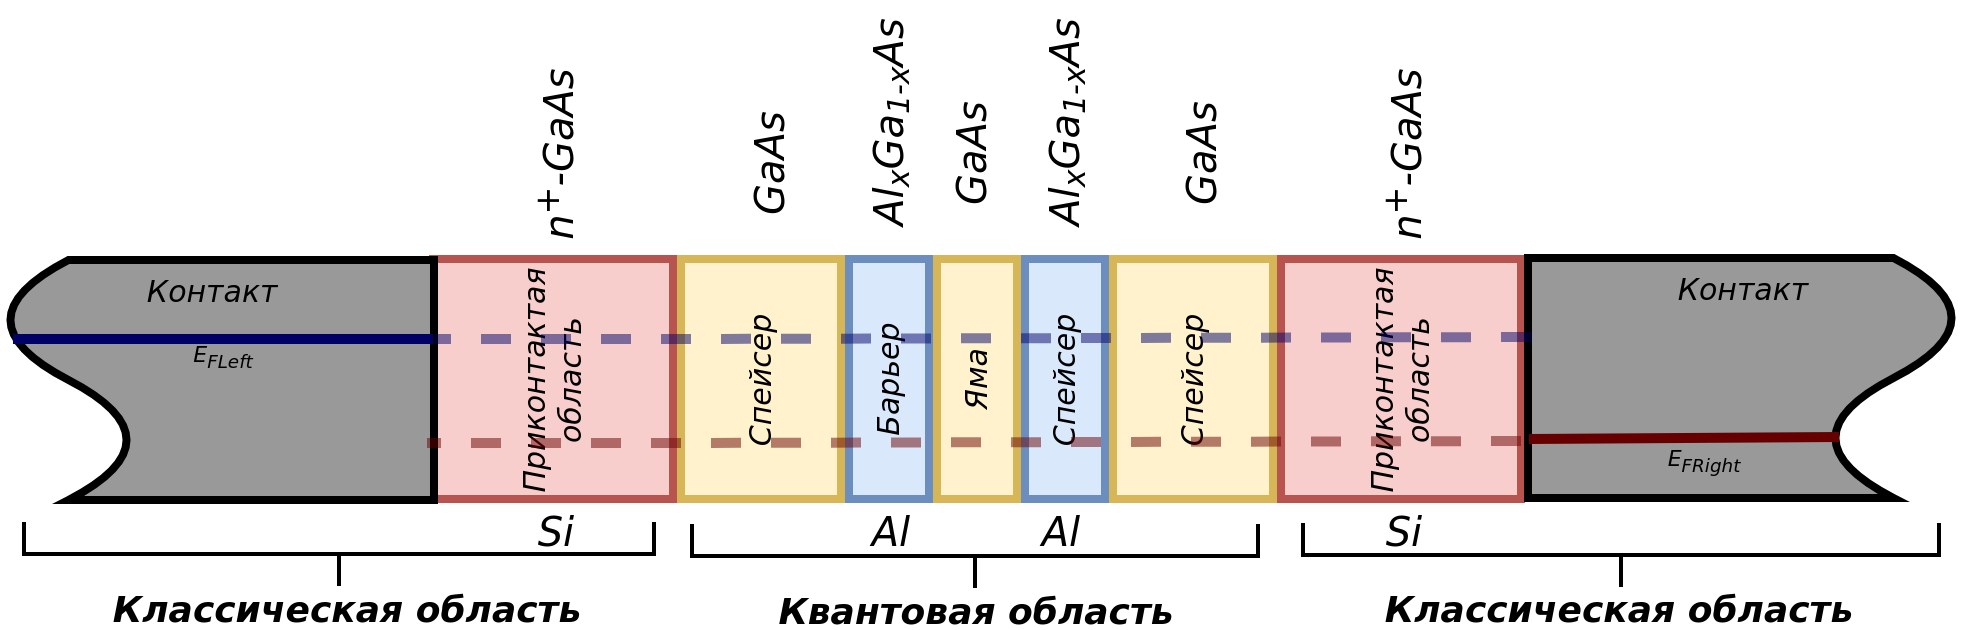
\includegraphics[width=0.9\linewidth]{assets/RTHSModelDiff}
	\caption{Стуктура РТГС для моделирования диффузии}
	\label{fig:RTHSModelDiff}
\end{figure}

В данной модели возможны:
\begin{itemize}
	\item Диффузия $Al$ из барьеров в яму;\\
	\item Диффузия $Si$ из приконтактных областей в активную область.
\end{itemize}

Рассмотрим диффузионное расплытие активной области и проникновение легирующий примеси отдельно.

\section{Дуффузионное расплытие активной области}
\begin{figure}[h]
	\centering
	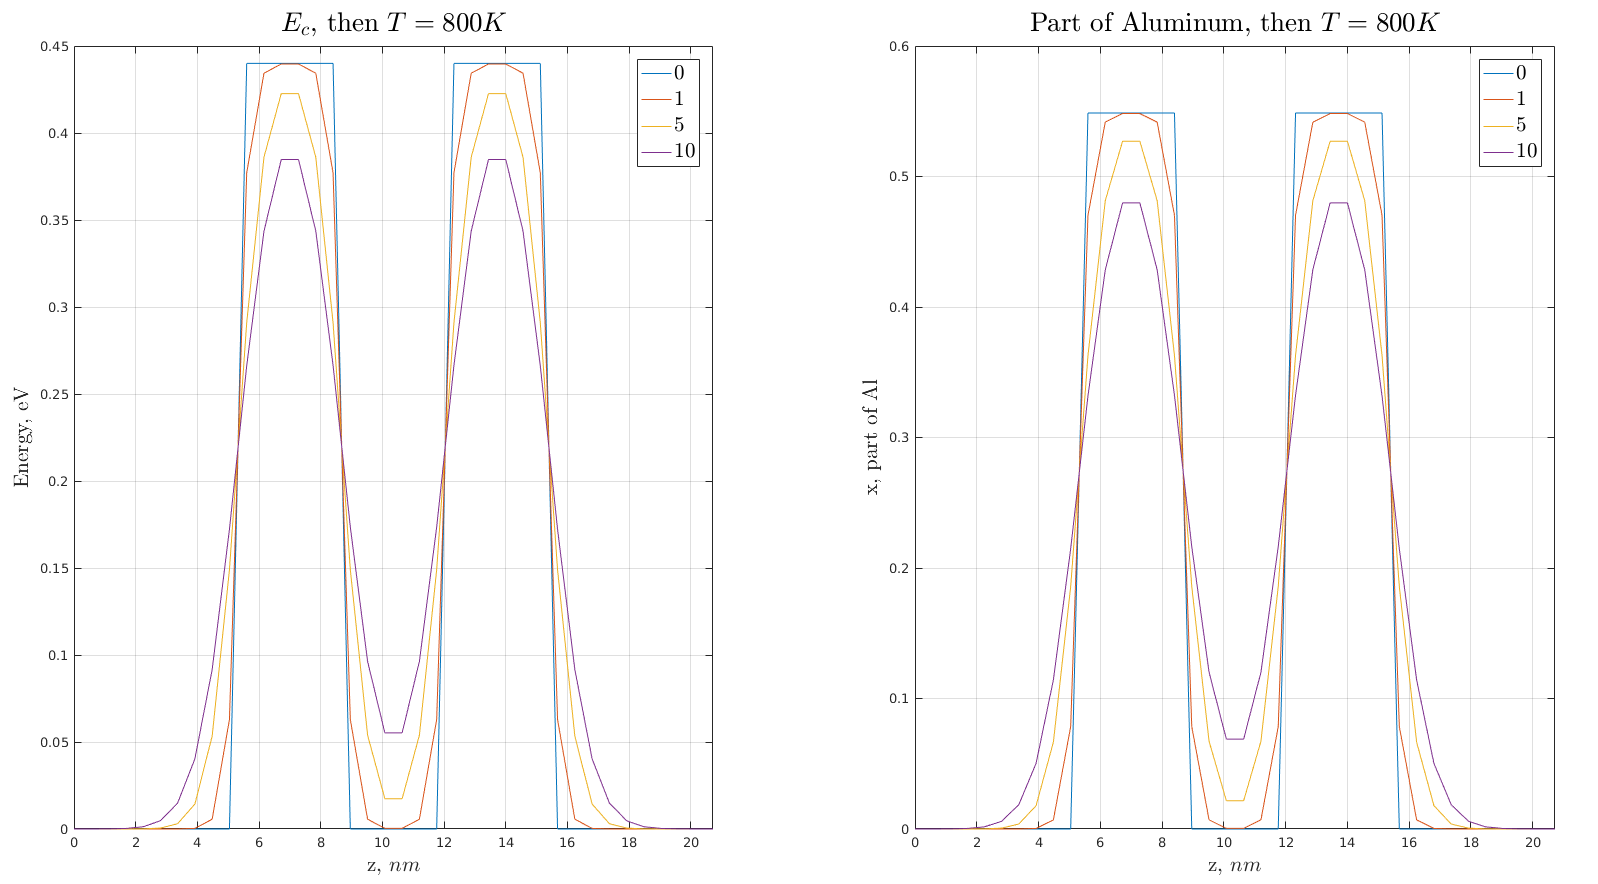
\includegraphics[scale=0.4]{DOAlGaAs}
	\caption{Расплытие потенциального рельефа чистого $Al_{x}Ga_{1−x}As$}
	\label{fig:DOAlGaAs}
\end{figure}

\begin{figure}[h]
	\centering
	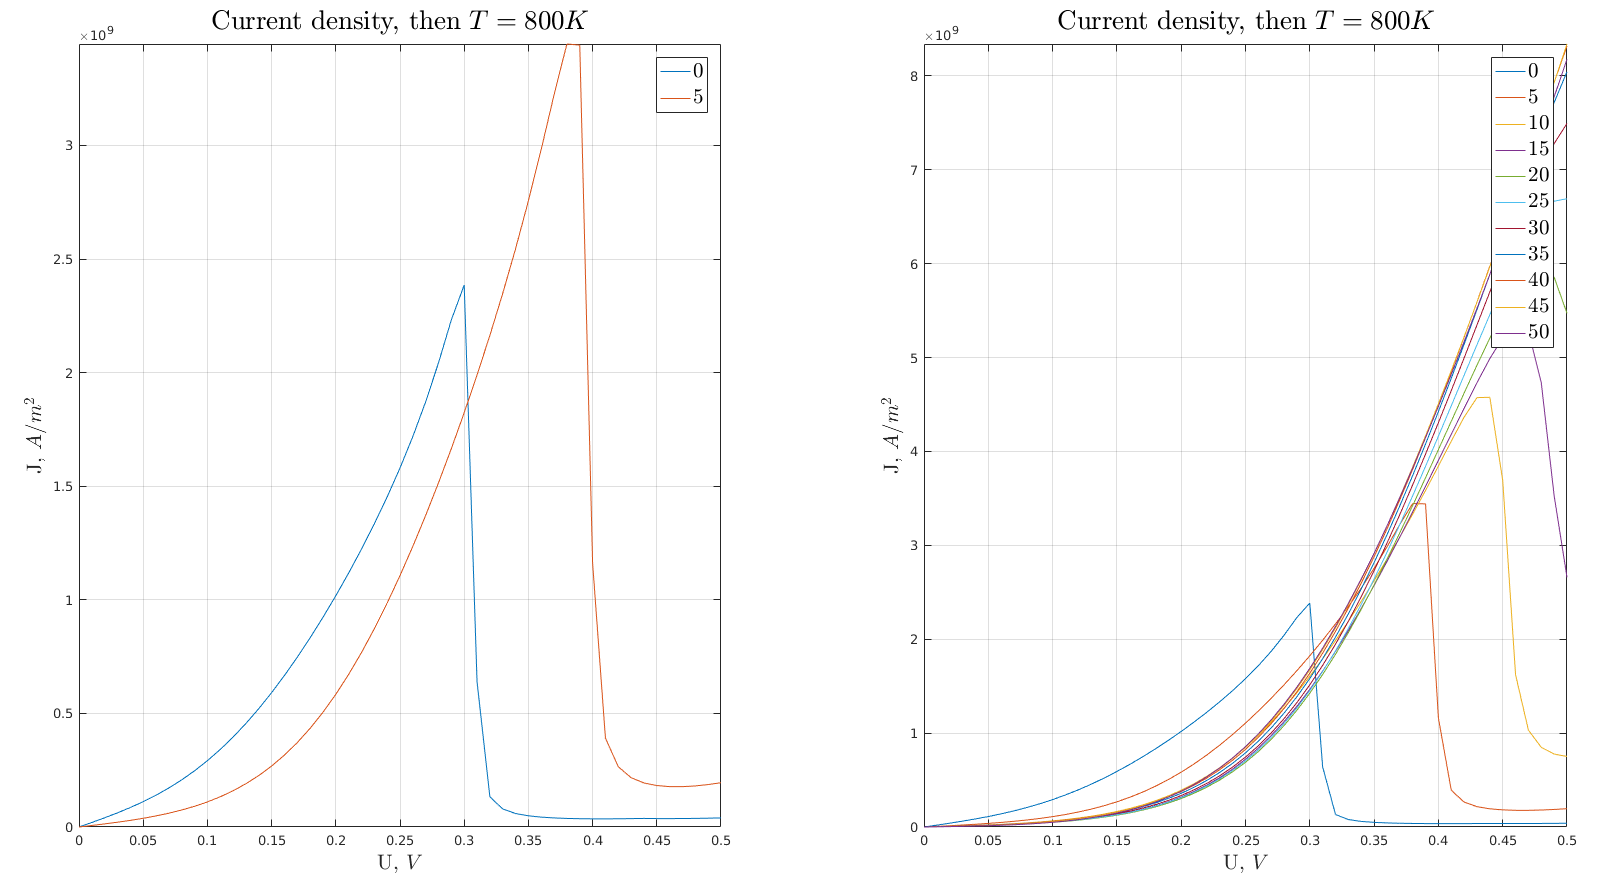
\includegraphics[scale=0.4]{JDOAlGaAs}
	\caption{Деградация тока через РГТС на основе чистого $Al_{x}Ga_{1−x}As$}
	\label{fig:JDOAlGaAs}
\end{figure}

\begin{figure}[h]
	\centering
	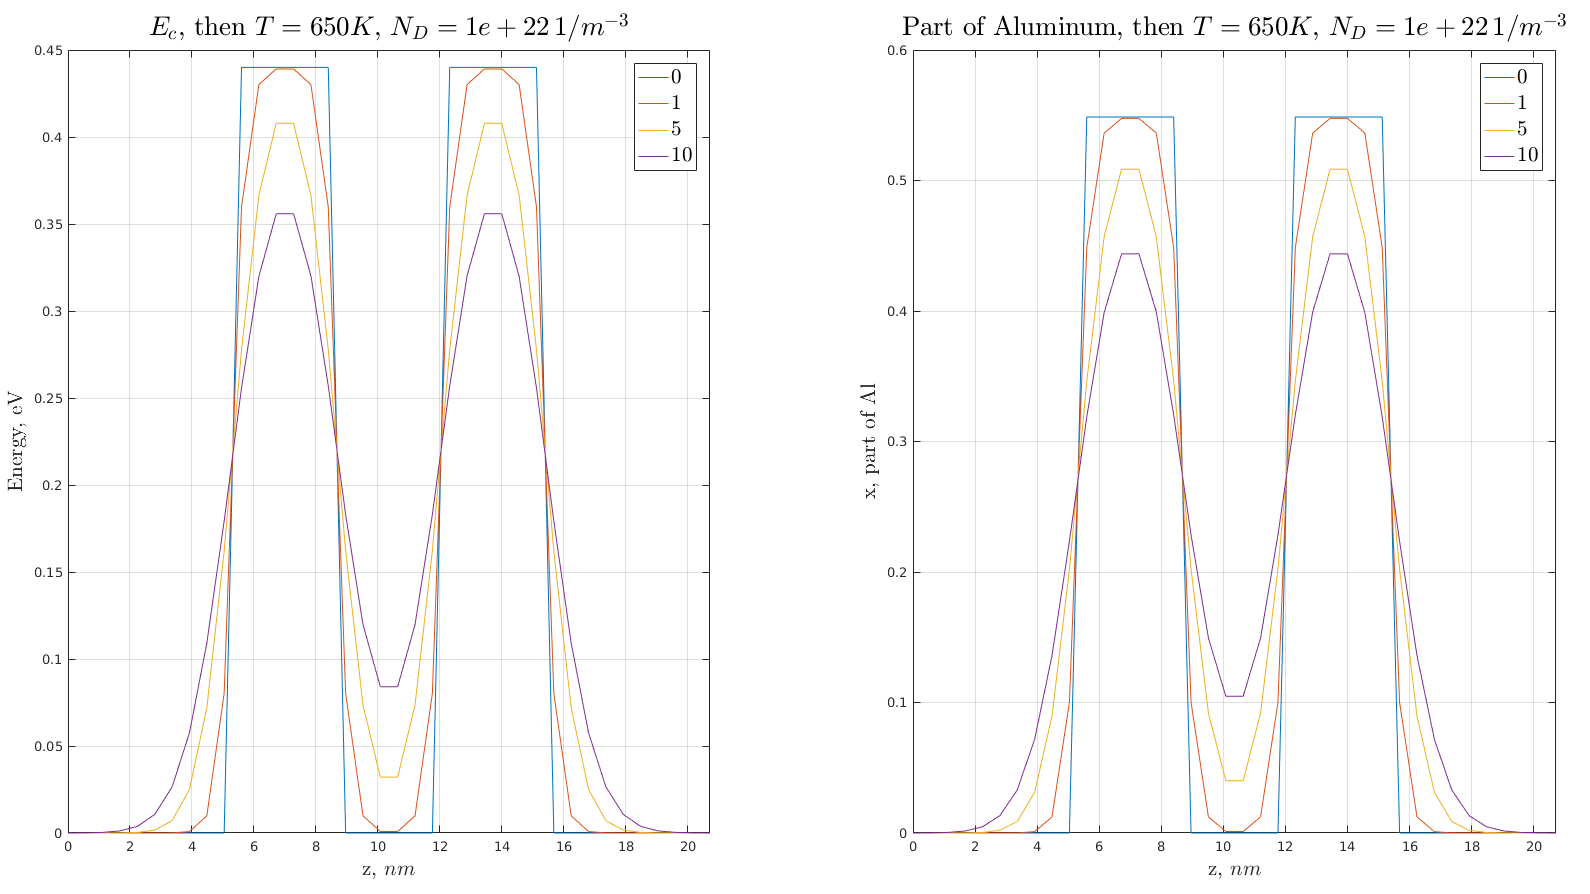
\includegraphics[scale=0.4]{DOAlGaAsNd}
	\caption{Расплытие потенциального рельефа $Al_{x}Ga_{1−x}As$ при наличии донорной примеси $N_{D}=1\,1/m^{-3}$} 
	\label{fig:DOAlGaAsNd}
\end{figure}

\begin{figure}[h]
	\centering
	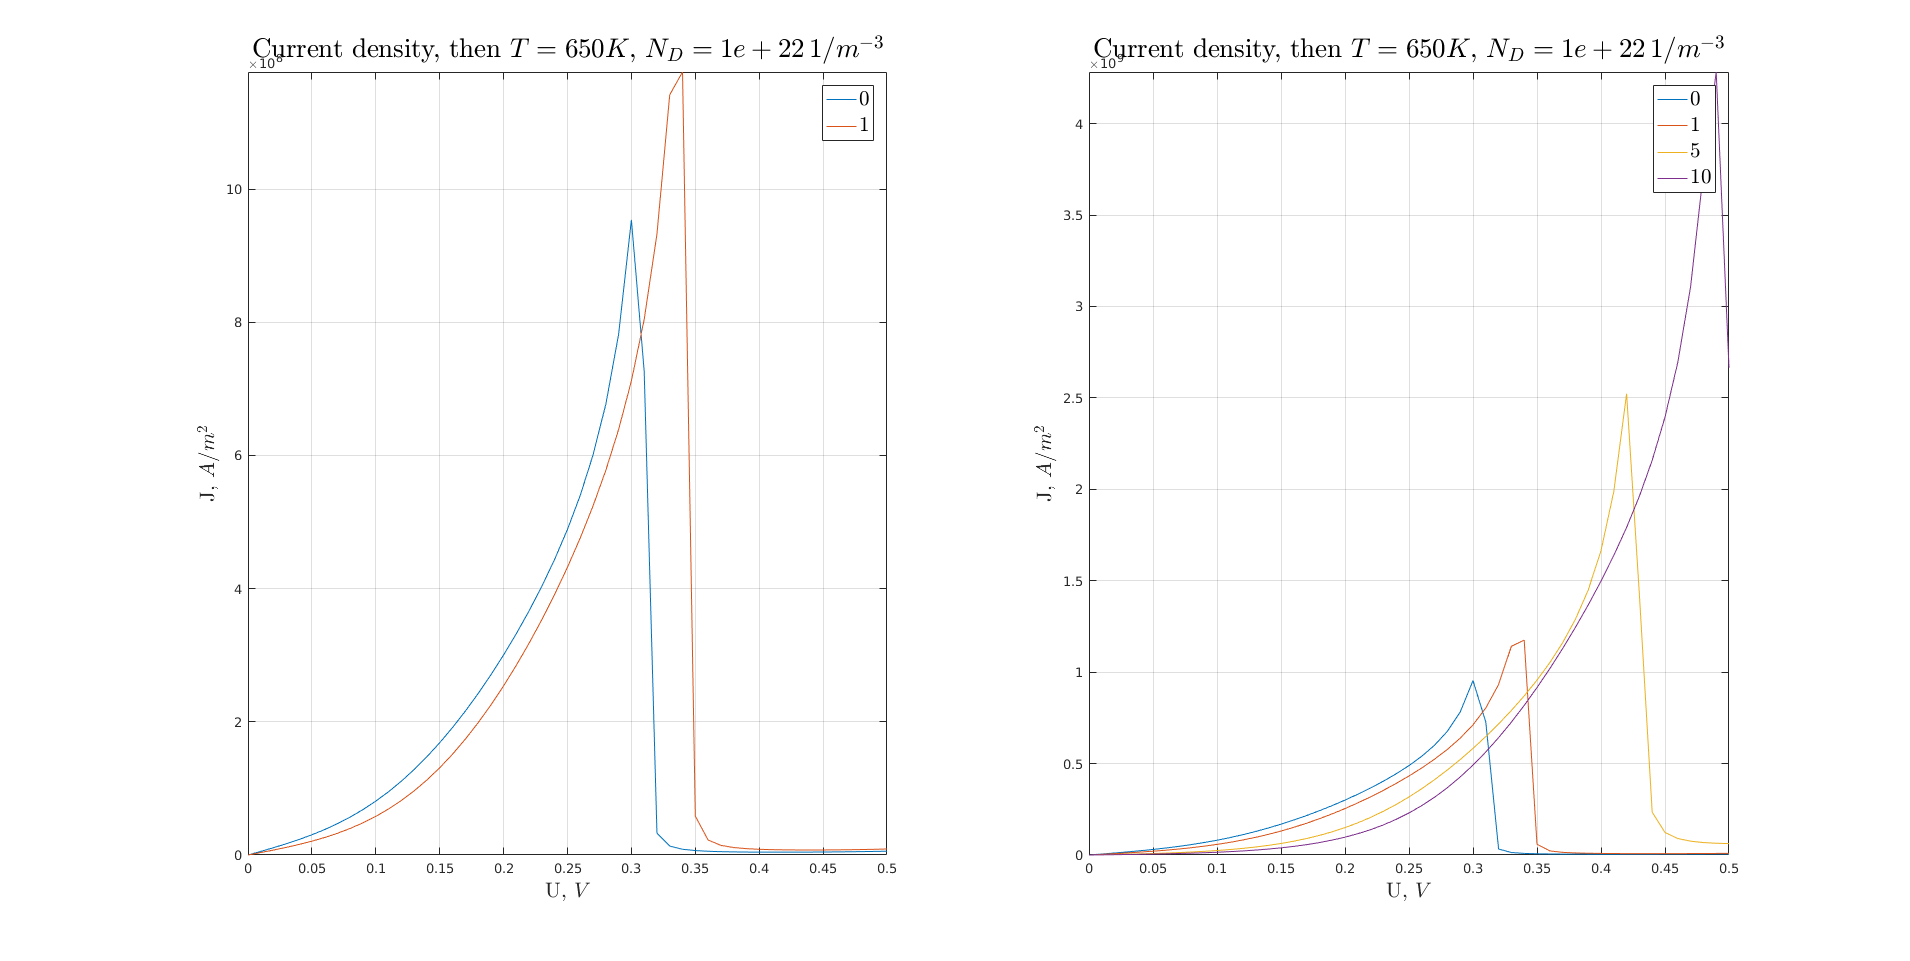
\includegraphics[scale=0.4]{JDOAlGaAsNd}
	\caption{Деградация тока через РГТС на основе $Al_{x}Ga_{1−x}As$ при наличии донорной примеси $N_{D}=1\,1/m^{3}$}
	\label{fig:JDOAlGaAsNd}
\end{figure}

\begin{figure}[h]
	\centering
	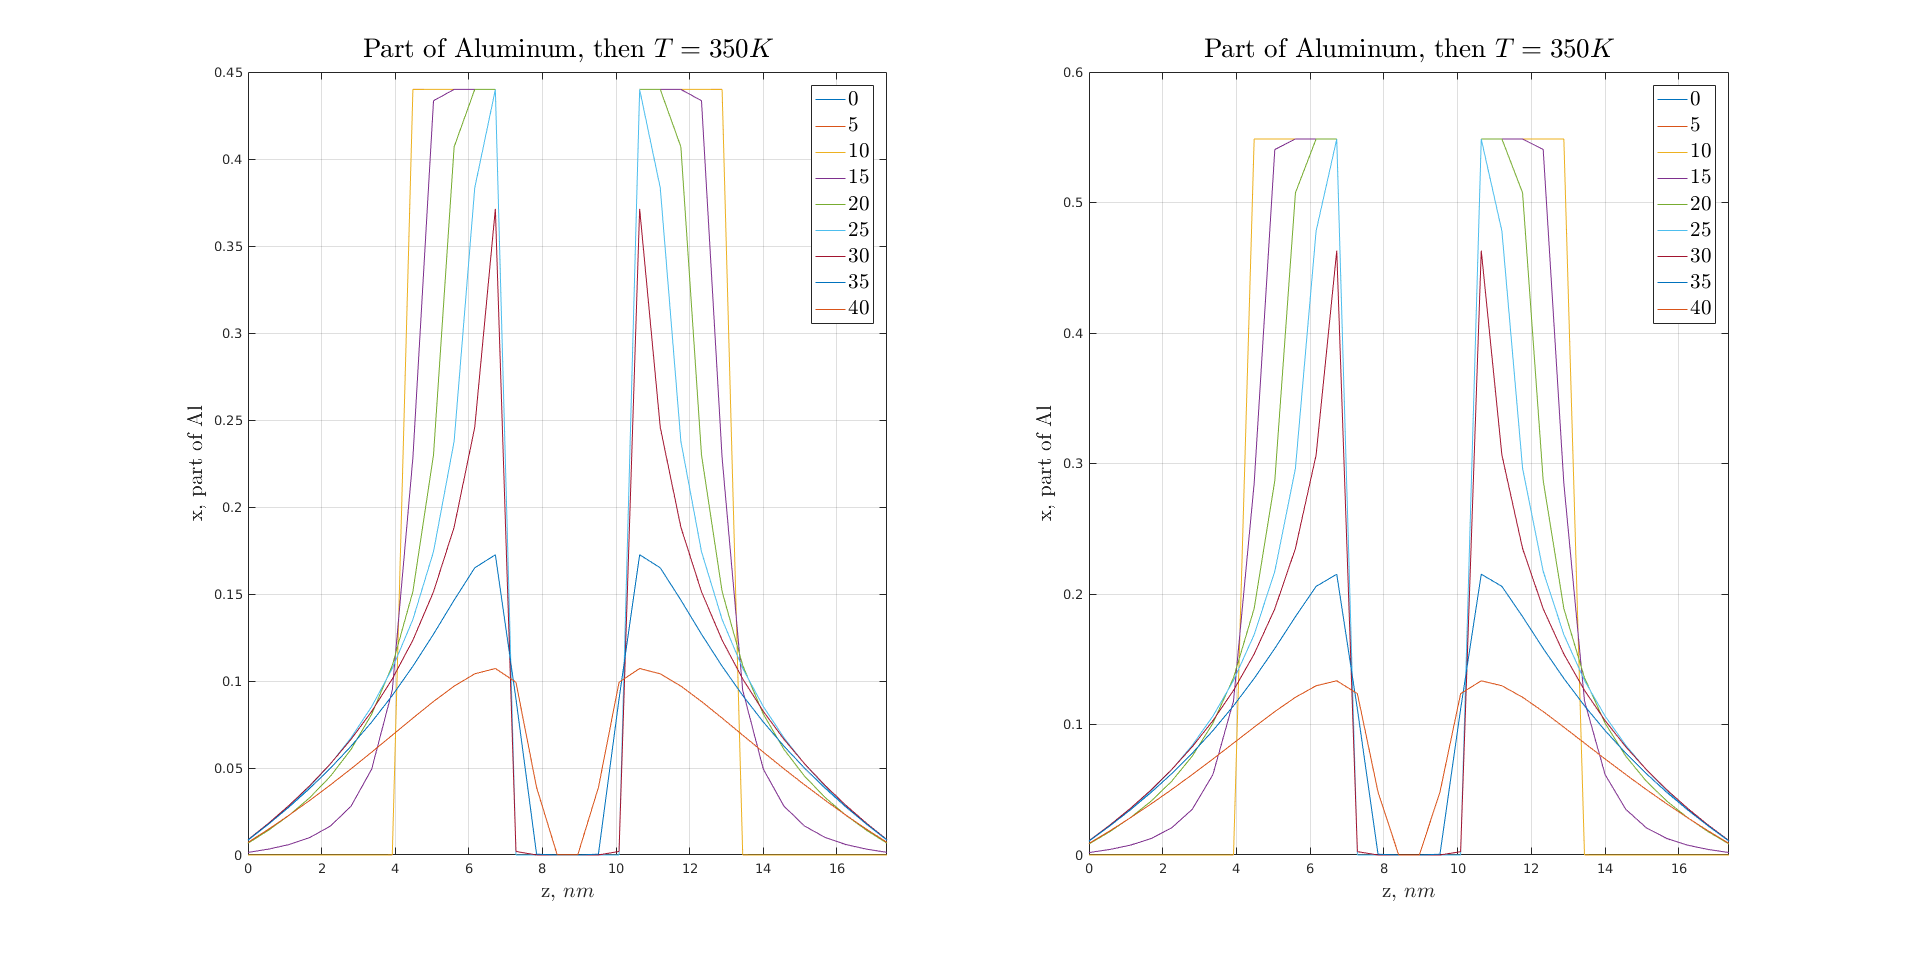
\includegraphics[scale=0.4]{DAlGaAs_Si}
	\caption{Расплытие потенциального рельефа $Al_{x}Ga_{1−x}As$ при наличии донорной примеси} 
	\label{fig:DAlGaAs_Si}
\end{figure}

\begin{figure}[h]
	\centering
	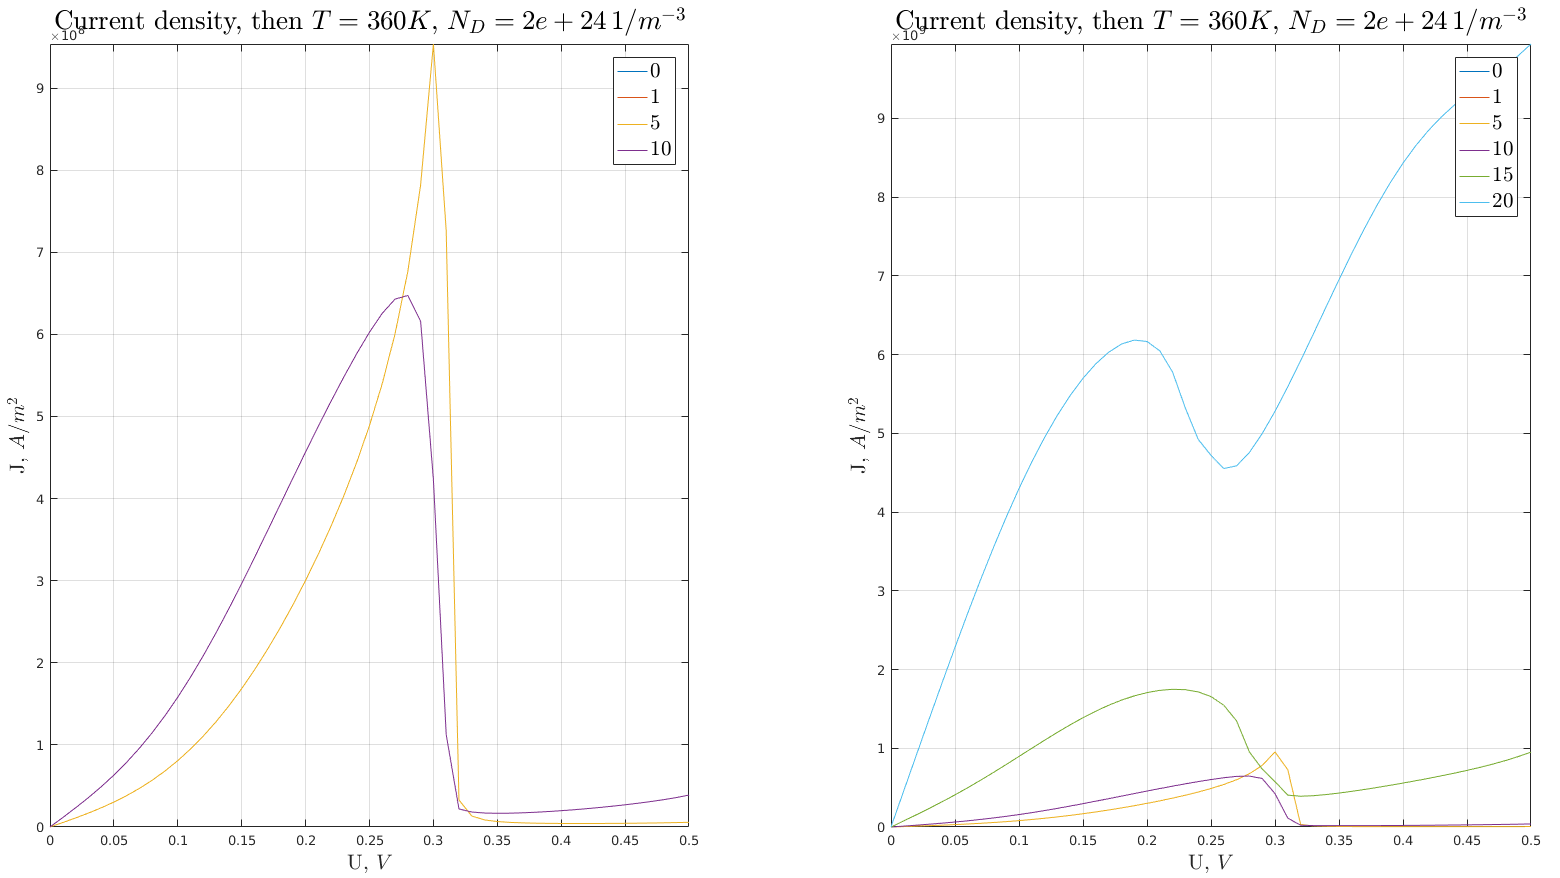
\includegraphics[scale=0.4]{JDAlGaAs_Si}
	\caption{Деградация тока через РГТС на основе $Al_{x}Ga_{1−x}As$ при наличии донорной примеси}
	\label{fig:JDAlGaAs_Si}
\end{figure}
